%-----------------------------------LICENSE------------------------------------%
%   This file is part of Mathematics-and-Physics.                              %
%                                                                              %
%   Mathematics-and-Physics is free software: you can redistribute it and/or   %
%   modify it under the terms of the GNU General Public License as             %
%   published by the Free Software Foundation, either version 3 of the         %
%   License, or (at your option) any later version.                            %
%                                                                              %
%   Mathematics-and-Physics is distributed in the hope that it will be useful, %
%   but WITHOUT ANY WARRANTY; without even the implied warranty of             %
%   MERCHANTABILITY or FITNESS FOR A PARTICULAR PURPOSE.  See the              %
%   GNU General Public License for more details.                               %
%                                                                              %
%   You should have received a copy of the GNU General Public License along    %
%   with Mathematics-and-Physics.  If not, see <https://www.gnu.org/licenses/>.%
%------------------------------------------------------------------------------%
%   Author:     Ryan Maguire                                                   %
%   Date:       February 28, 2023                                              %
%------------------------------------------------------------------------------%
\documentclass{beamer}
\usepackage{amsmath}

\title{Newtonian Black Holes}
\author{Ryan Maguire}
\date{January 24, 2023}
\usenavigationsymbolstemplate{}
\setbeamertemplate{footline}[frame number]
\begin{document}
    \maketitle
    \begin{frame}{Outline}
        \begin{itemize}
            \item Classical Mechanics
            \item Black Holes
            \item Euler's Method
            \item Runge-Kutta Method
            \item Raytracing
            \item Cool Pictures
        \end{itemize}
    \end{frame}
    \begin{frame}{Classical Mechanics}
        It's been known for some time that the speed of light is not infinite.
        Newton observed that a finite light speed would explain discrepancies
        in orbits of Jupiter's moons with the classical theory of gravity.
        This observation can accurately compute the speed of light as well.
    \end{frame}
    \begin{frame}{Classical Mechanics}
        Nothing in classical mechanics says there is a universal speed limit,
        and there is no indication that the speed of light itself must be
        constant.
        \par\hfill\par
        The original idea of \textit{aether} tries to model light after sound,
        and sound can have variable speed depending on the medium it is
        travelling through. We'll abuse this a lot to get a very rough
        estimate of a black hole as far as Newtonian mechanics is concerned.
        It is not a physically realistic assumption.
    \end{frame}
    \begin{frame}{Classical Mechanics}
        If you take a ball and throw it in the air, it comes back. If you had
        an absolute cannon of an arm, perhaps you could throw the ball at
        11,186 meters per second. It would certainly go a lot high, but would
        it ever come back?
    \end{frame}
    \begin{frame}{Classical Mechanics}
        Let's use the universal law of gravitation, which is a classical law
        (no general relativity here), but is accurate in many scenarios.
        The potential energy is given by an inverse law:
        \begin{equation}
            U=-\frac{GMm}{r}
        \end{equation}
        Where $G$ is the universal gravitational constant, $M$ is the mass of
        the earth, $m$ is the mass of the ball, and $r$ is the distance from
        the ball to the center of the earth. Kinetic energy is given by:
        \begin{equation}
            K=\frac{1}{2}mv^{2}
        \end{equation}
        where $v$ is the speed (norm of velocity) of the speed.
    \end{frame}
    \begin{frame}{Classical Mechanics}
        Let's try to throw the ball at a speed such that the ball will slow
        down to 0 m/s \textit{at infinity}. The potential energy at infinity is
        zero, since $\frac{1}{r}\rightarrow{0}$ as $r\rightarrow\infty$.
        Invoking conservation of energy:
        \begin{align}
            U_{0}+K_{0}&=U_{\infty}+K_{\infty}\\
            U_{0}+K_{0}&=0+0\\
            -\frac{GMm}{R}+\frac{1}{2}mv_{0}^{2}&=0\\
            v_{0}=\sqrt{\frac{2GM}{R}}
        \end{align}
        Where $R$ is the radius of the Earth.
        This value $v_{0}$ is \textit{escape velocity}, the speed at which is
        needed for an object to \textit{escape} the influence of a bodies
        gravitational pull.
    \end{frame}
    \begin{frame}{Black Holes}
        In the previous slides we were considering the Earth. The radius was
        constant, as was the mass, and we solved for the escape velocity.
        Instead, let's suppose the mass $M$ is
        fixed, and the \textit{escape velocity} $v_{0}$ is constant as well.
        The variable to solve for is the radius $R$.
        \begin{equation}
            R=\frac{2GM}{v_{0}^{2}}
        \end{equation}
        What would happen if we chose $v_{0}=c$, the speed of light
        (ignore the title of this current slide, please)?
    \end{frame}
    \begin{frame}{Black Holes}
        The result is a black hole. The gravitational pull is so strong that
        even light can't escape, so the result is blackness. The formula
        obtained is the \textit{Schwarzschild radius}:
        \begin{equation}
            R=\frac{2GM}{c^{2}}
        \end{equation}
        Fun-fact, this is the same formula you get after doing all the
        rigorous general relativity calculations
        (Assuming a few conditions, such as the black hole is not rotating).
        \par\hfill\par
        We're going to try and draw a black hole using the world of classical
        mechanics.
    \end{frame}
    \begin{frame}{Euler's Method}
        Given a vector-valued ordinary differential equation:
        \begin{equation}
            \frac{\textrm{d}\mathbf{r(t)}}{\textrm{d}t}
            =f\big(\mathbf{r(t)}\big)
        \end{equation}
        one of the simplest means of solving this numerically is
        \textit{Euler's method}. Replacing the differentials with small
        displacements, we get:
        \begin{equation}
            \frac{\Delta\mathbf{r}(t)}{\Delta{t}}
            \approx{f}\big(\mathbf{r}(t)\big)
        \end{equation}
    \end{frame}
    \begin{frame}{Euler's Method}
        Given initial conditions $\mathbf{r}(t_{0})=\mathbf{r}_{0}$ we can
        further expand this as follows:
        \begin{align}
            \Delta\mathbf{r}(t)&\approx{f}\big(\mathbf{r}(t)\big)\Delta{t}\\
            \mathbf{r}(t_{0}+\Delta{t})-\mathbf{r}(t_{0})
            &\approx{f}\big(\mathbf{r}(t_{0})\big)\Delta{t}\\
            \mathbf{r}(t_{1})&\approx\mathbf{r}(t_{0})+
                f\big(\mathbf{r}(t_{0})\big)\Delta{t}
        \end{align}
        as $\Delta{t}$ gets smaller, the accuracy of the approximation improves.
        We then obtain a sequence $\mathbf{r}_{n}$ of approximate values of
        $\mathbf{r}(t_{n})$:
        \begin{equation}
            \mathbf{r}(t_{n+1})\approx\mathbf{r}(t_{n})+
                f\big(\mathbf{r}(t_{n})\big)\Delta{t}
        \end{equation}
    \end{frame}
    \begin{frame}{Euler's Method}
        The previous slide is great for first order differential equations,
        but the equations of motions in classical mechanics deal with
        second order vector-valued differential equations. This stems from
        Newton's second law:
        \begin{equation}
            \mathbf{F}=m\mathbf{a}
                =m\frac{\textrm{d}^{2}\mathbf{r}(t)}{\textrm{d}t^{2}}
        \end{equation}
        where $\mathbf{a}(t)$ is the acceleration, and $\mathbf{F}$ is the
        force.
    \end{frame}
    \begin{frame}{Euler's Method}
        Let's extend Euler's method to second order differential equations.
        \begin{equation}
            \frac{\textrm{d}^{2}\mathbf{r}(t)}{\textrm{d}t^{2}}
                =f\big(\mathbf{r}(t)\big)
        \end{equation}
        with initial conditions $\mathbf{r}(t_{0})$ and
        $\dot{\mathbf{r}}(t_{0})$ known to us.
        We start by defining the velocity:
        \begin{equation}
            \mathbf{v}(t)=\frac{\textrm{d}\mathbf{r}(t)}{\textrm{d}t}
        \end{equation}
        The differential equations can be approximated by:
        \begin{equation}
            \frac{\Delta\mathbf{v}(t)}{\Delta{t}}
            \approx{f}\big(\mathbf{r}(t)\big)
        \end{equation}
        so long as the time step $\Delta{t}$ is small.
    \end{frame}
    \begin{frame}{Euler's Method}
        We mimic the method from before and obtain:
        \begin{equation}
            \mathbf{v}(t_{1})=\mathbf{v}(t_{0})
                +f\big(\mathbf{r}(t_{0})\big)\Delta{t}
        \end{equation}
        where $\mathbf{v}(t_{0})=\dot{\mathbf{r}}(t_{0})$. We can now update
        the position vector:
        \begin{equation}
            \mathbf{r}(t_{1})
                =\mathbf{r}(t_{0})+\mathbf{v}(t_{0})\Delta{t}
        \end{equation}
        And in general, we obtain two sequences:
        \begin{align}
            \mathbf{v}(t_{n+1})&=\mathbf{v}(t_{n})
                +f\big(\mathbf{r}(t_{n})\big)\Delta{t}\\
            \mathbf{r}(t_{n+1})
                &=\mathbf{r}(t_{n})+\mathbf{v}(t_{n})\Delta{t}
        \end{align}
        This idea immediately extends to higher order differential equations.
        The local error in these methods is roughly proportional to the square
        of the step size $\Delta{t}$. The global error grows linearly.
    \end{frame}
    \begin{frame}{Runge-Kutta Method}
        The raytracing we'll do for black holes uses Euler's method with a
        lot steps (hundreds of thousands) with a small $\Delta{t}$. We would be
        able to use a larger step size if the error bounds were proportional to
        higher powers of $\Delta{t}$, and this is where the Runge-Kutta method
        comes in to play.
        \par\hfill\par
        For the sake of time, I won't give the derivation (which is much
        longer than Euler's method), but remark that the error is
        proportional to $\Delta{t}^{4}$. The Runge-Kutta programs required
        far fewer iterations, while achieving similar accuracy.
    \end{frame}
    \begin{frame}{Results}
        \begin{figure}
            \centering
            \resizebox{0.7\textwidth}{!}{%
                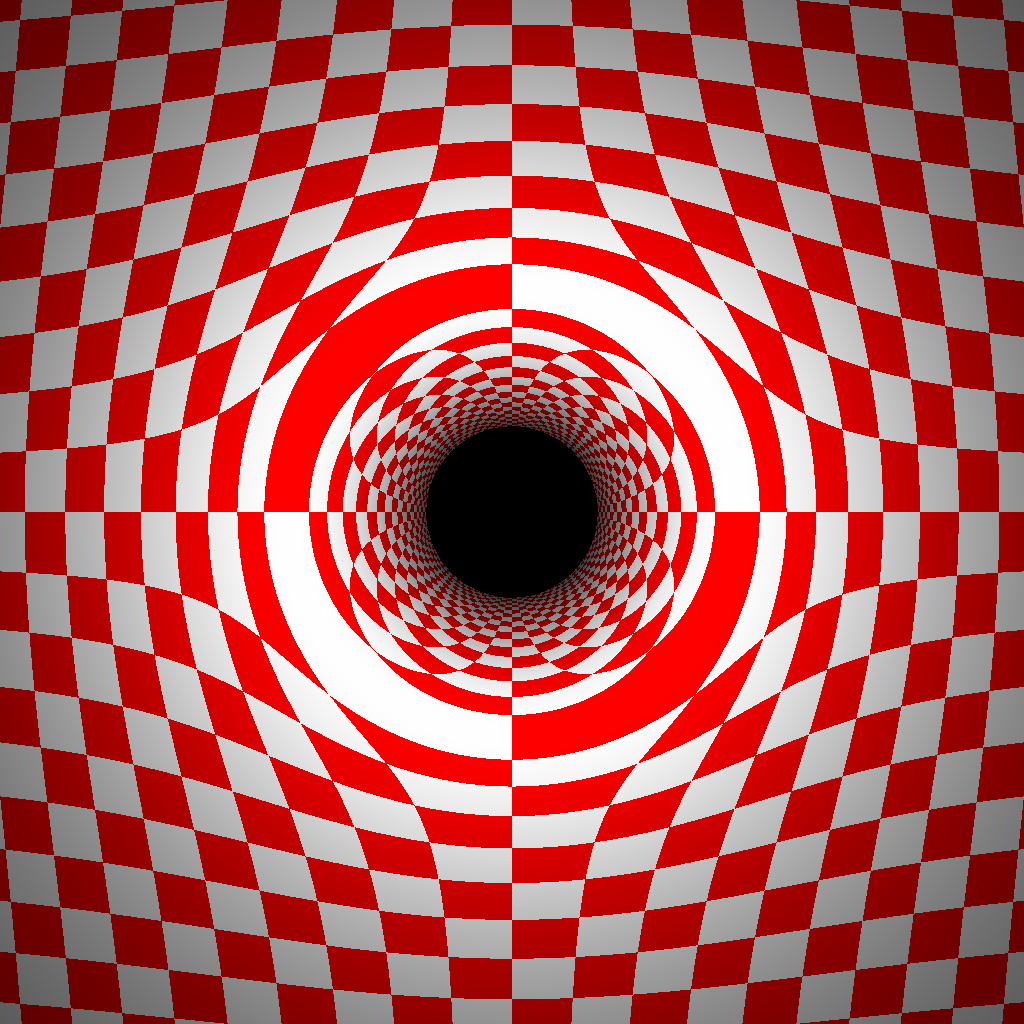
\includegraphics{../images/newtonian_black_hole.png}
            }
        \end{figure}
    \end{frame}
    \begin{frame}{Results}
        \begin{figure}
            \centering
            \resizebox{0.7\textwidth}{!}{%
                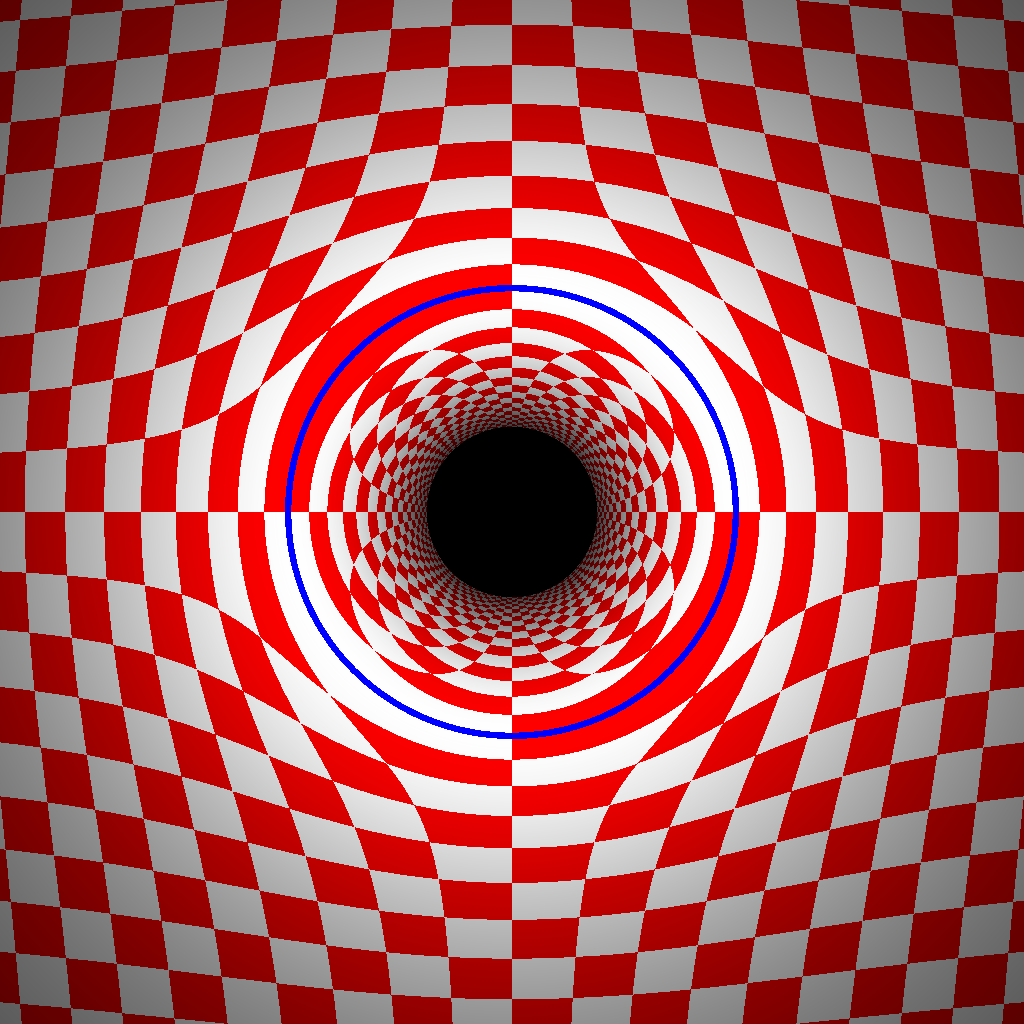
\includegraphics{../images/newtonian_black_hole_center_highlight.png}
            }
        \end{figure}
    \end{frame}
    \begin{frame}{Results}
        \begin{figure}
            \centering
            \resizebox{0.7\textwidth}{!}{%
                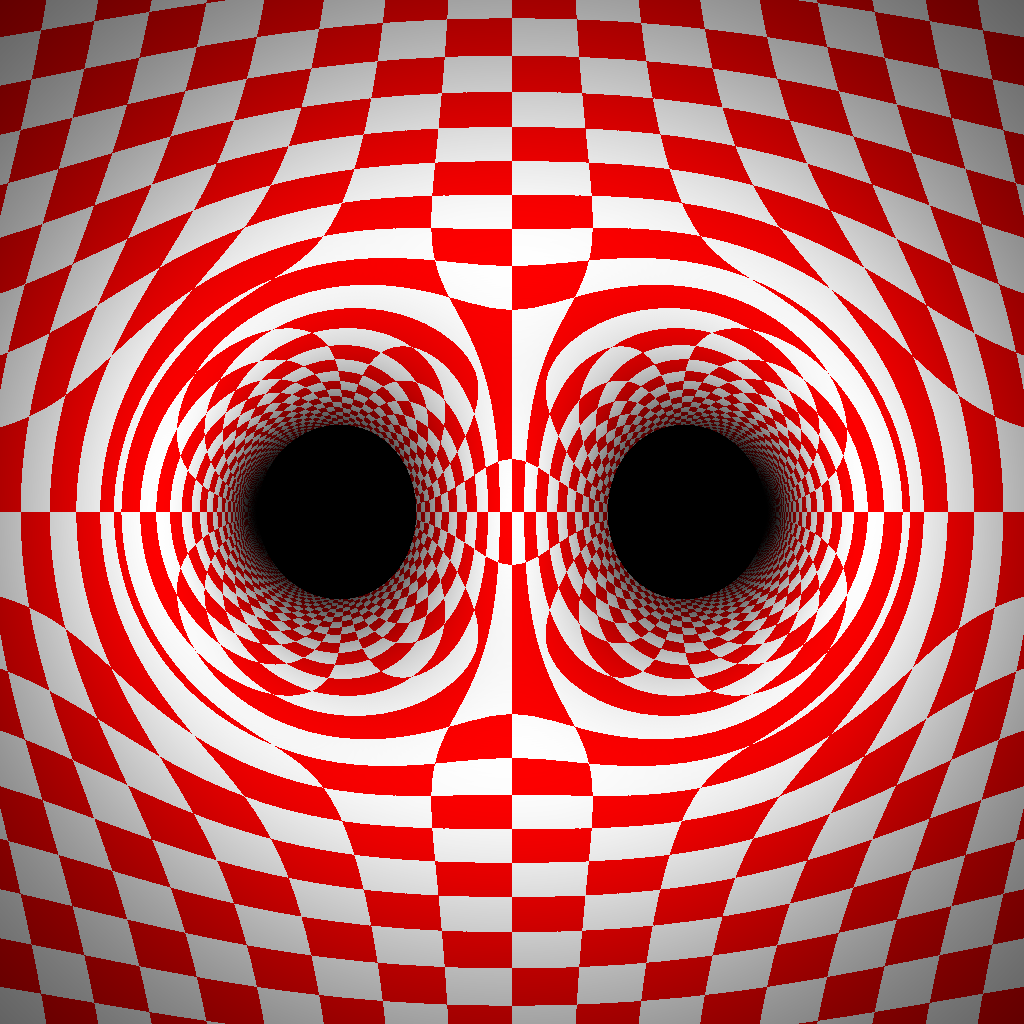
\includegraphics{../images/newtonian_black_hole_two.png}
            }
        \end{figure}
    \end{frame}
    \begin{frame}{Results}
        \begin{figure}
            \centering
            \resizebox{0.7\textwidth}{!}{%
                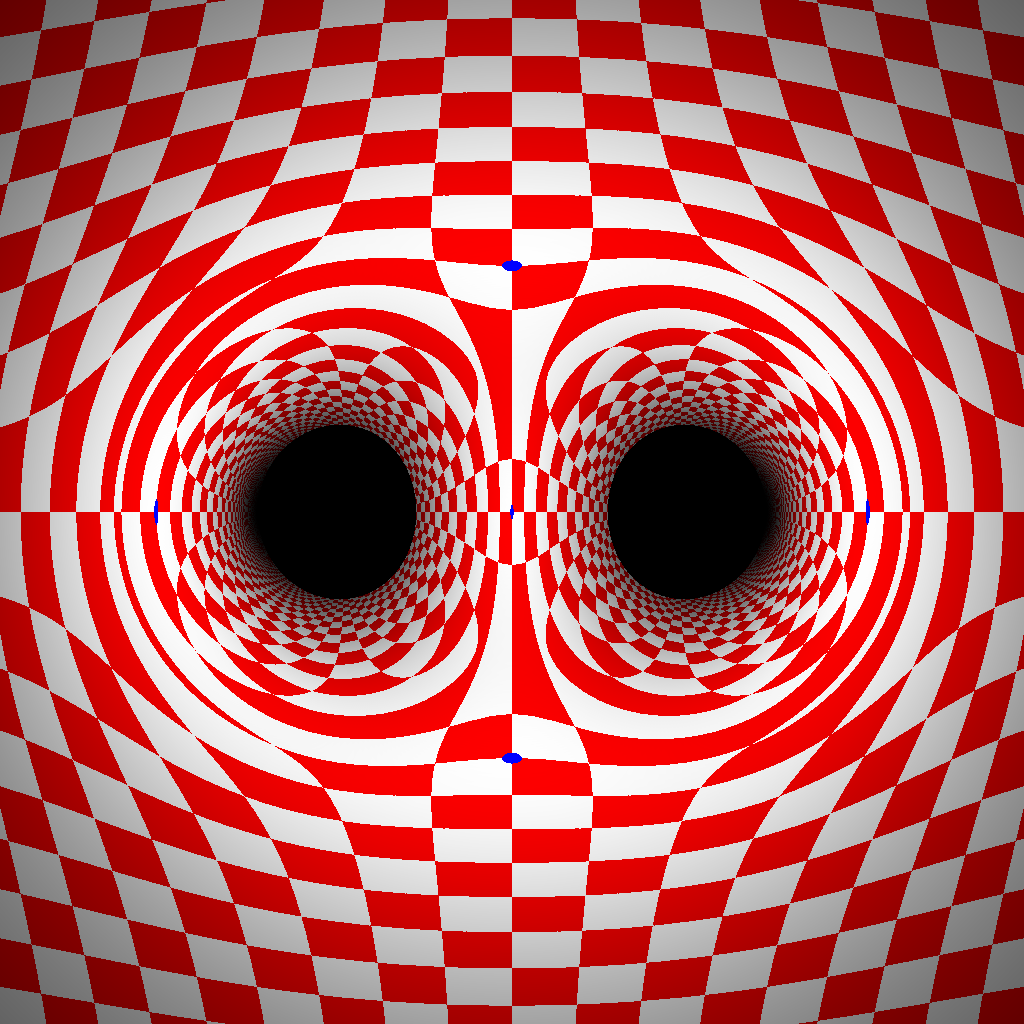
\includegraphics{../images/newtonian_black_hole_two_center_highlight.png}
            }
        \end{figure}
    \end{frame}
    \begin{frame}{Results}
        \begin{figure}
            \centering
            \resizebox{0.7\textwidth}{!}{%
                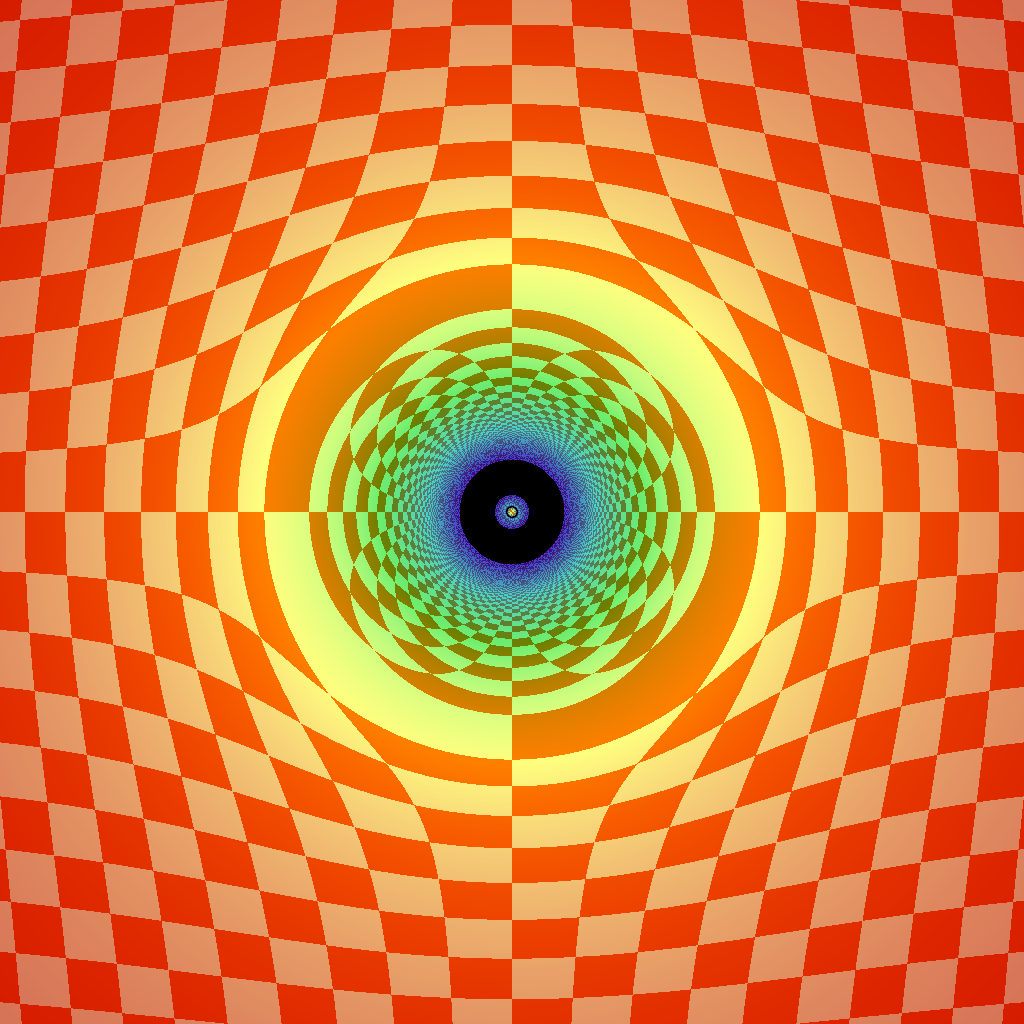
\includegraphics{../images/newtonian_black_hole_point_source_rainbow.png}
            }
        \end{figure}
    \end{frame}
    \begin{frame}{The End}
        \begin{center}
            Thanks!
        \end{center}
    \end{frame}
\end{document}
